\chapter{Giới thiệu đề tài}
\pagestyle{fancy}
    \section{Giới thiệu}
    Với sự gia tăng nhanh chóng của số lượng phương tiện giao thông, con người ngày càng cần những hệ thống thông minh hơn cho việc quản lý hàng tá phương tiện giao thông này. Đóng một phần quan trọng trong hệ thống này đó là những ứng dụng liên quan đến nhận dạng biển số bởi tính thiết thực của chúng. Hiện đã có nhiều nghiên cứu cũng như áp dụng những hệ thống nhận dạng biển số trong việc quản lý bãi xe, phát hiện vi phạm giao thông, hệ thống thu phí tự động... Các hệ thống nhận dạng biển số thương mại nổi tiếng có thể kể đến là OPENALPR hay SIGHTHOUND.

    Hệ thống nhận dạng biển số gồm ba giai đoạn cơ bản nhất đó là: xác định vị trí của biển số, phân tách các kí tự trên biển số và nhận diện các kí tự đó. Trong đó, giai đoạn đầu tiên giữ vai trò vô cùng quan trọng. Nó cần độ chính xác rât cao thậm chí là hoàn hảo bởi việc xác định sai vị trí của biển số sẽ dẫn đến hậu quả cho những giai đoạn tiếp theo. Nhiều giải pháp đã được áp dụng cho giai đoạn này (sử dụng xử lý ảnh hay áp dụng những giải thuật học máy,...) nhằm giảm thời gian xử lí cũng như giảm tỉ lệ lỗi.

    Với xử lí ảnh, phương pháp này phụ thuộc rất nhiều vào điều kiện thực tế như là ánh sáng, ảnh nền, độ rõ nét của hình ảnh, góc nhìn hay loại biển số (xe gắn máy, ô tô, xe buýt,...).

    Với áp dụng các giải thuật học máy (ví dụ: YOLO) là một hướng tiếp cận theo hiệu quả. Nó khắc phục được những hạn chế của các giải thuật thuần xử lí ảnh. Giải pháp này yêu cầu sự đầy đủ của tập dữ liệu cho đào tạo và sức mạnh phần cứng rất lớn bởi hàng tá những phép toán tích chập nhiều lớp. Sự phát triển của GPUs đã đáp ứng được yêu cầu về phần cứng. OPENALPR, SIGHTHOUND đều được hiện thực và chạy trên nền tảng GPUs. Tuy nhiên vần còn nhiều hạn chế về giá cả, hiệu năng,...

    Trong đề tài này nhóm sẽ tiếp cận bài toán theo hướng sử dụng giải thuật học máy chạy trên nền tảng hệ thống vi mạch không đồng nhất (FPGAs). Với những ưu điểm về giá thành, hiệu năng,... của FPGAs cùng với sức mạnh tính toán khá lớn hiện nay, nhóm quyết định thực hiện đề tài nhằm kiểm thử tính khả thi của hướng tiếp cận này.
    \section{Giới hạn đề tàit}
    
    
    \section{Sơ đồ khối và hoạt động}
    \textbf{Sơ đồ khối} (Hình \ref{fig:sysblockdiagram})
    \begin{figure}[htp]
    		\centering
     		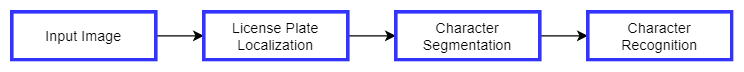
\includegraphics[scale=.55]{images/sys_block_diagram.png}
    		\caption{Sơ đồ khối của hệ thống}
    		\label{fig:sysblockdiagram}
    	\end{figure}
    \textbf{Hoạt động}